\section{Méthodes possibles pour la virtualisation légère}
\label{section:emulation}

Il existe actuellement deux méthodes permettant de faire de la virtualisation
légère. La première est une émulation par limitation ou dégradation également
appelée virtualisation standard et la seconde est une émulation par
interception.

\subsection{Virtualisation standard}
%% \begin{itemize}
%% \item principe: limiter l'accès aux ressources par exemple (cgroup, netstat, cpuburner), temps d'un SEB (bench avec netlink, limiter (cap))
%% \item avantage plus simple
%% \item désavantages: host>>target, modèle à vérifier, contrôle expérimental fin
%% \end{itemize}
Avec cette première méthode on place la couche d'émulation au-dessus de la
plate-forme réelle (comme un hyperviseur pour une VM). De fait, la puissance de
l'émulateur dépend de la puissance de la machine hôte et ne peux pas dépasser
les capacités de cette dernière. En effet, des machines plus puissantes que
l'hôte répondrait plus rapidement que ce dernier à une demande d'une
application. Or le délai de réponse géré par l'émulateur ne peut-être inférieur
à celui de l'hôte sinon l'hôte n'aurait pas le temps de faire les calculs
demandés et de répondre à l'émulateur qui répondrait à l'application. De plus,
en choisissant de placer l'émulation comme une sur-couche cela permet de limiter
l'accès aux ressources pour les applications. En effet les applications ne
pourront pas passer la couche d'émulation pour accéder aux ressources localisées
sur la machine hôte. Les requêtes des applications distribuées seront arrêtées
par l'émulateur. C'est lui qui s'occupera de récupérer les ressources demandées
par les applications. Il existe différent outils permettant de faire de mettre
en place cette virtualisation, on trouve notamment \textbf{cgroup},
\textbf{netstat} et \textbf{cpuburner}.  Cette solution à l'avantage d'être
simple à mettre en \oe uvre puisque l'on se basse sur la machine hôte. Néanmoins
elle est assez contraignante du fait qu'on ne puisse pas émuler des
architectures plus performantes que l'hôte. De plus {\color{red} à écrire deux
  derniers points négatifs à éclaircir}.

\subsection{Émulation par interception}
%% principe: interception des actions et médiation (pas juste interception et rejeu). Intercepter des symboles pour en changer l'effet

Dans le cas de l'émulation par interception, pour faire croire à l'application
qu'elle s'exécute sur une machine autre que l'hôte on va utiliser deux outils;
un simulateur pour virtualiser l'environnement d'exécution et une API qui va
attraper toutes les communications de l'application avec l'hôte et qui les
transmettra ensuite au simulateur. Les calculs de l'application seront
effectués sur la machine hôte mais c'est le simulateur qui calculera le temps de
réponse à l'application. Pour cela il fera un rapport entre le temps d'exécution
du calcul sur la machine hôte (fourni par l'API), la puissance de l'hôte et
celle des machines de l'environnement que l'on simule. Le temps de l'application
sera donc celui du simulateur et non le temps réel. En effet, l'application
quand elle fait un calcul pense être sur une autre machine avec des performances
différentes, elle est donc capable de savoir combien de temps prends une certain
calcul sur son architecture. Hors sur l'hôte ce calcul ne prendra pas le même
temps et l'application se retrouvera avec un temps prévu et un temps qui ne
correspondent pas ce qui est problématique.  Avec cette solution on ne se
contente pas de faire de l'interception d'action et du rejeu par l'émulateur
comme c'est le cas avec l'émulation par limitation. On va intercepter les
actions des applications et faire de la médiation, autrement dit on va modifier
les actions avant de les laisser s'exécuter sous le contrôle de l'émulateur.

 Une application distribuée peut vouloir communiquer avec l'hôte soit pour
 effectuer de simples calculs (SEB), soit pour effectuer des requêtes de
 connexion ou de communication avec d'autres applications sur le réseau. Quand
 l'émulateur intercepte une communication venant d'un des processus d'une
 application, il modifie les caractéristiques de cette dernière pour qu'elle
 puisse s'exécuter sur la machine hôte. Quand la machine hôte renvoie une
 réponse à l'application, elle est également interceptée par l'émulateur pour
 que l'application ne voit pas le changement d'architecture. En même temps, il
 envoie au simulateur des données concernant le temps d'exécution de l'action
 sur la machine hôte pour qu'il puisse calculer le temps d'exécution sur la machine simulée. Les délais
 calculés par le simulateur sont soit des temps de calculs soit des temps de
 connexion. \textit{Quand le simulateur a terminé le calcul du temps de réponse
 nécessaire il l'envoie à l'émulateur qui l'envoie à l'application en plus du résultat afin de mettre à
 jour l'horloge de l'application.} Ainsi les calculs sont réellement exécuter
 sur la machine, les communications réellement émises sur le réseau géré par le
 simulateur et c'est le temps de réponse fourni par le simulateur qui va
 influencer l'horloge de l'application permettant ainsi d'imiter un
 environnement distribué. Finalement les applications ne communiquent plus
 directement entre elles puisque toute communication est interceptée par
 l'émulateur, puis gérée par le simulateur qui s'occupe du réseau.

{\color{red} Mettre deux schémas de action interceptes, test modifie, renvoie,
  attrape réponse, simulateur, retour application, un quand simple calcul l'autre quand connexion}

Pour intercepter ces actions, il faut d'abord choisir à quel niveau se place
l'interception: code source ou binaire. Mais il faut également choisir sur quel
type de symbole utilisée par l'application pour exécuter ses actions se fera la
médiation qui suit l'interception et avec quel outil. En effet une application
peut communiquer avec le noyau via différentes abstractions. Elle peut soit
utiliser les fonctions d'interaction directe avec le noyau que sont les appels
systèmes, soit utiliser les différentes abstractions fournies par le système
d'exploitation: bibliothèques (fonctions systèmes de la libc par exemple) ou les
fonctions POSIX dans le cas d'un système UNIX.

\begin{figure}[H]
 \centering
 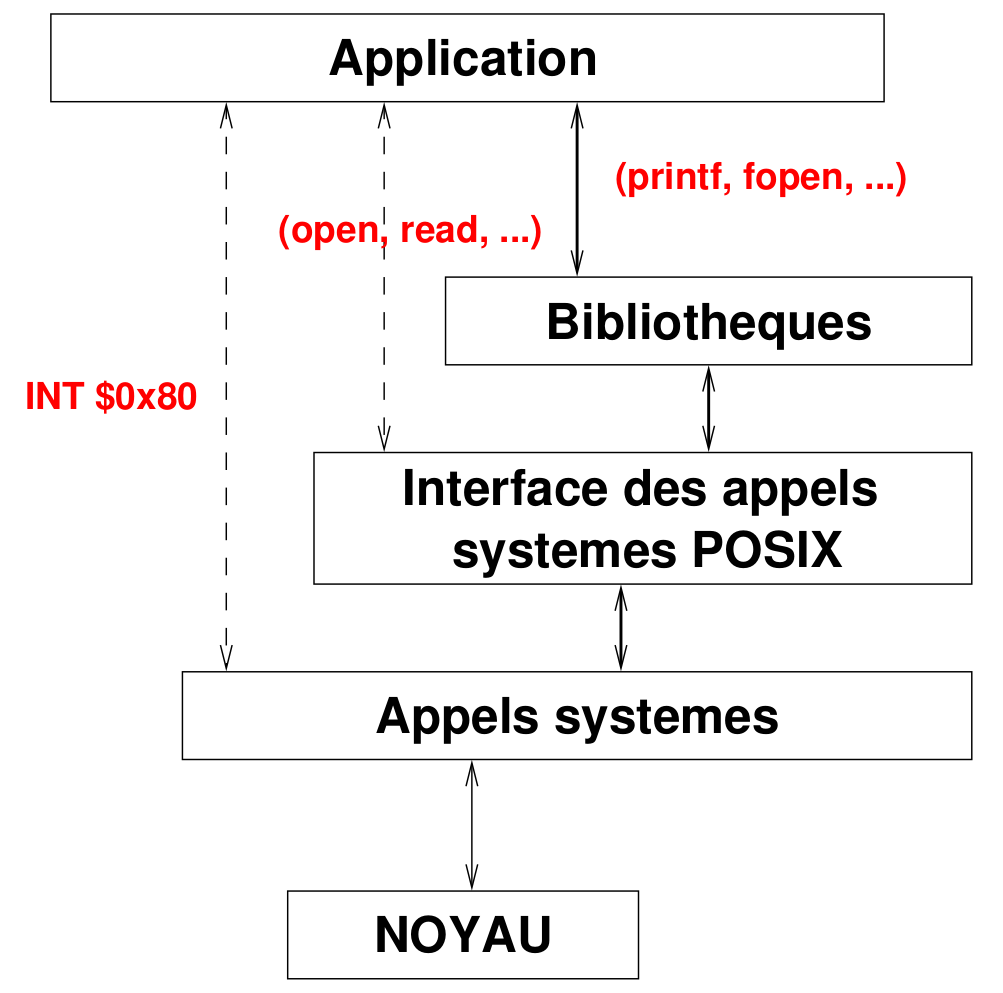
\includegraphics[scale=0.5]{Pictures/Communication_application_noyau.png}
 \caption{Communications possibles entre le noyau et une application}
 \label{AS_Communication}
\end{figure}

Nous allons donc voir comment on peut faire de l'interception sur un fichier source puis sur un binaire, puis nous verrons comment faire de la médiation sur différents symboles: appels de fonctions et appels systèmes.
%% {\color{red} L'interception des actions d'une application peut se faire à deux niveaux: sur le fichier source et sur le binaire. La médiation qui suit l'interception des actions peut également se faire sur différent type de symboles: les appels de focntions et les appels systèmes.  \textit{mettre partie ce qu'on intercepte pourquoi et le schéma}}

\subsubsection{Action sur le fichier source}
%% reimplem SMPI (trop spé) ,source to source/ pass LLVM( gcc+libc=consanguin) 
%% , Coccinelle
\subsubsection{Action sur le binaire}
%%Valgrind (perf pourrie)
  

    

\subsubsection{Médiation des Appels Système}
%% pourquoi: read/write, comm reseau 

En regardant la Fig.\ref{AS_Communication}, et les différents niveaux
d'abstractions, le moyen plus simple pour attraper les actions de l'application
en gérant un minimum de choses serait d'intercepter directement les appels
systèmes.  Les appels systèmes sont constitués de deux parties; la première,
l'entrée, initialise l'appel via les registres de l'application qui contiennent
les arguments de l'appel puis donne la main au noyau. La seconde, la sortie,
inscrit le retour de l'appel système dans le registre de retour de
l'application, les registres d'arguments contenant toujours les valeurs reçues à
l'entrée de l'appel système, et rend la main à l'application. Nous devons donc
intercepter les deux parties de l'appel système pour maintenir notre
environnement simulé et donc stopper l'application à chaque fois pour récupérer
ou modifier les informations nécessaires avant de lui rendre la main pour entrer
ou sortir de l'appel système.

 Nous allons donc voir comment il est possible de faire cela, puisque de
 nombreux outils existent {\color{red}et si cette solution se suffit à elle
   même.}
 
 \paragraph{L'API ptrace}\cite{INTERCEPTION:AS, INTERCEPTION:MARION},
 qui est lui même un appel système permet de tracer tous les événement désirés
 d'un processus, mais aussi d'écrire et de lire directement dans l'espace
 d'adressage de ce dernier, à n'importe quel moment ou lorsque un événement
 particulier se produit selon le choix du processus. De cette façon il peut
 contrôler l'exécution d'un processus. C'est un appel système unique dont chaque
 action à effectuer est passée sous forme de requêtes en paramètre de l'appel
 système.

Pour pouvoir contrôler un processus via ptrace on va créer deux processus parent
via un \textit{fork()}; un processus exécutera l'application et qu'on souhaite
contrôler, appelé ``processus espionné'' et l'autre processus le contrôlera, il
se sera appelé ``processus espion''. Le processus espionné indiquera au
processus espion qu'il souhaite être contrôlé via un appel système ptrace et une
requête PTRACE\_TRACEME puis il exécutera l'application via un
\textit{exec()}. À la réception de cet appel le processus espion notifiera son
attachement au processus espionné via un autre appel à ptrace et une requête
PTRACE\_ATTACH. Il indiquera également sur quelles actions du processus espionné
il veut être notifié (chaque instruction, signal, sémaphore...), définissant
ainsi les actions bloquantes pour le processus espionné. Dans notre cas, ce
seront les appels systèmes que l'on considérera comme point d'arrêt pour le
processus espionné, ainsi le processus espion sera appelé deux fois: à l'entrée
et à la sortie de l'appel système. Ainsi quand un des processus de l'application
voudra faire un appel système quelconque il sera bloqué avant de l'exécuter,
l'appel système ptrace sera lancé et notifiera le processus espion. Ce dernier
fera les modifications nécessaires dans les registres du processus espionné pour
conserver la virtualisation de l'environnement grâce aux requêtes PEEK\_DATA et
POKE\_DATA passées en argument de l'appel système. Puis il rendra la main au
processus espionné bloqué pour que l'appel système puisse avoir lieu. Au retour
de l'appel système le processus espionné sera de nouveau stoppé, un ptrace sera
envoyé au processus espion qui remodifiera les informations nécessaires. Puis il
rendra la main au processus espionné bloqué qui sortira de son appel système
avec un résultat exécuté sur la machine hôte et un temps d'exécution et une
horloge fournie par le simulateur. Quand un processus espion a fini un suivi, il
peut envoyer deux types de requêtes au processus espionné: PTRACE\_KILL qui
termine le processus espionné ou PTRACE\_DETACH qui le laisse continuer son
exécution.

{\color{red} Mettre un schéma attachement attente père attrape signal
  modification main fils as retour père...}

Néanmoins, pour contrôler un processus ptrace fait de nombreux changements de
contexte pour pouvoir intercepter et gérer les événements. De plus il supporte
mal les processus utilisant du multithreading, et ne fait pas parti de la norme
POSIX donc son exécution peut varier d'une machine à une autre.

\paragraph{Uprobes}\cite{INTERCEPTION:AS, INTERCEPTION:MARION}
%% Non module noyau
pour \textit{user-space probes}, quant à lui est une API noyau, également appelé
module d'instrumentation, permettant d'insérer dynamiquement des points d'arrêts
à n'importe quel endroit dans le code d'une application, dans notre cas les
appels systèmes. Pour chaque point d'arrêt l’utilisateur fournit un handler
particulier à exécuter avant ou après l’instruction marquée. Uprobes étant un
outil s'exécutant dans le noyau les handlers doivent être des modules. Pour
chaque point d'arrêt géré par Uprobes, on a donc un module noyau qui contient le
handler à exécuter, ainsi que le processus et l'adresse virtuelle du point
d'arrêt. Lorsqu'un point d'arrêt est atteint Uprobes prend la main et exécute le
bon handler. Pour savoir qu'un point d'arrêt a été touché Uprobes utilise Utrace
équivalent de ptrace en mode noyau qui permet d'éviter les nombreux changements
de contexte et qui est capable de gérer le multithreading. Utrace peut également
être utilisé dans le module gérant un point d'arrêt pour récupérer des
informations sur l'application et les données qu'elle utilise.

Les deux avantages de l'API noyau est qu'elle est rapide et qu'elle a accès à
toutes les ressources sans aucune restriction. Mais ce dernier point représente
aussi son plus gros défaut de par sa dangerosité. De plus, dans notre cas il ne
semble pas judicieux de faire de la programmation noyau via des modules dont il
faudra également gérer le bon chargement.

\paragraph{seqcomp/bpf}
%% Read only



%%Malgré ses défauts c'est donc l'appel système ptrace qui a été choisi.
%% {\color{red} \textbf{gérer cette transition}} Néanmoins il a été montré dans un
%% précédent stage que l'appel système ptrace est inefficace voir inutile en ce qui
%% concerne tous les appels systèmes temporels qu'une application voudrait
%% faire. \textit{les appels systèmes ``time'', ``clock\_gettime'',
%%   ``gettimeofday'' avec \textbf{ptrace} ne sont pas possibles, d'où l'alliance
%%   avec LD\_PRELOAD} Par exemple lors d'un gettimeofday l'appel système n'est pas
%% lancé on répond directement au niveau de la bibliothèque ainsi on n'arrive même
%% pas au niveau de l'appel système, donc ptrace ne fait rien.  Problème
%% portabilité {\color{red} \textbf{gérer cette transition}}
\subsubsection{Médiation directe des appels de fonctions}
%%pourquoi: pthread, temps
\paragraph{linker: LD\_PRELOAD}
%pas suid
%% On pourrait alors penser qu'une bonne solution serait d'intercepter les actions
%% de l'application au niveau des bibliothèques.{\color{red} rajouter des trucs sur
%%   VDSO}. Pour cela il existe la variable d'environnement \textbf{LD\_PRELOAD}
%% qui contient la liste des bibliothèques à précharger et qui est utilisée par le
%% noyau lors du premier lancement d'un programme. En effet par défaut Linux
%% effectue une édition de lien dynamique, l'édition de lien statique n'étant
%% choisie qu'en l'absence de bibliothèques partagées définissant les fonctions
%% utilisées par l'application. On va donc créer notre propre bibliothèque de
%% fonctions surchargeant chaque fonction susceptible d'être utilisée par
%% l'application. Une fonction surchargée contiendra alors toutes les modifications
%% nécessaires pour maintenir notre environnement simulé suivi de l'appel à la
%% fonction initiale puisqu'on souhaite juste intercepter l'appel et pas
%% l'empêcher. On préchargera cette bibliothèque avant les autres en la plaçant
%% dans la variable LD\_PRELOAD, ainsi nos fonctions passeront avant les fonctions
%% des bibliothèques usuelles.

%% Néanmoins si l'application fait un appel système directement sans passer par la
%% couche \textit{Bibliothèques} Fig.~\ref{AS_Communication} notre mécanisme
%% d'interception est contournée. En effet on ne peut surcharger que des fonctions
%% avec cette solution, pas des appels systèmes. De même si on oublie de réécrire
%% une fonction d'une des bibliothèques utilisée par l'application. Cette solution
%% n'est donc pas suffisante pour le modèle d'interception que nous souhaitons
%% avoir.

%% Cependant on peut voir que LD\_PRELOAD résout les problèmes de ptrace concernant
%% les fonctions de temps, et inversement puisque ptrace permet d'intercepter les
%% appels systèmes que le modèle d'interception avec LD\_PRELOAD ne permet pas de
%% gérer. Une solution choisie lors d'un précédent stage est donc d'allier les
%% deux. On surchargera les fonctions temporelles dans notre bibliothèque
%% préchargée avec LD\_PRELOAD pour pallier les lacunes temporelles de ptrace. Et
%% pour toutes les autres fonctions ptrace s'en occupera, ainsi on est certain de
%% n'oublier aucune fonction. Maintenant que nous savons ce que nous devons
%% intercepter et comment l'intercepter nous allons voir ce que nous devons
%% modifier pour pouvoir maintenir notre émulation simulation.

%% \textit{Pour faire face à ce problème il a été choisi d'utiliser l'éditeur de
%%   lien dynamique \textbf{LD\_PRELOAD}, ce dernier intercepte les appels de
%%   l'application au niveau des bibliothèques. Pour cela on va créer une
%%   bibliothèque.}

\paragraph{linker got injection}
%% plus dur que nécessaire   

{\color{red} \textit{petit tableau comparatif}}
